\documentclass[12pt]{exam}

\newcommand{\ds}{\ensuremath{\displaystyle}}

\usepackage{amsmath,amsfonts, amsthm}
\usepackage{multicol}
\usepackage{multirow}
\usepackage{harpoon}
\renewcommand{\arraystretch}{1.5}

\newcommand{\harpvec}[1]{\overrightharp{\ensuremath{\mathbf{#1}}}}
\newcommand{\vect}[1]{\harpvec{#1}}
\newcommand{\<}{\langle}
\renewcommand{\>}{\rangle}

% ref: http://pgfplots.sourceforge.net/gallery.html
% ref: http://tex.stackexchange.com/a/74575/79754
\usepackage{pgfplots}% This uses tikz
\pgfplotsset{compat=newest}% use newest version
\tikzset{LineStyle/.style={smooth, ultra thick, samples=400}}

% \printanswers

\begin{document}

\begin{center}
\fbox{\fbox{\parbox{5.5in}{\centering
MATH 1121 - Fall 2015 - Dr. Clontz - Test 1
}}}
\end{center}
\vspace{0.1in}
\makebox[\textwidth]{
  Name:\enspace\hrulefill\hrulefill\hrulefill\space
  Section:\enspace\hrulefill\space
}

\vspace{12pt}

\begin{itemize}
  \item This test is worth 250 points toward your overall grade.
        Each problem is labeled with its value toward this total.
  \item On multiple choice problems, you do not need to show your work. No
        partial credit will be given.
  \item On full response problems, show all of your work and give a
        complete solution. When in doubt, don't skip any steps. Partial
        credit will be given at the discretion of the instructor.
  \item This exam is open notes, provided that these notes are completely
        in your own handwriting. The professor may take up notes you use
        with your test and return them after the test is graded.
  \item Tests submitted after the end of 70 minutes will be docked 25 points,
        with 25 points deducted every following minute.
\end{itemize}

\newpage

\begin{center}
  \textbf{Multiple Choice (150 points total)}
\end{center}

\begin{questions}

\setcounter{question}{0}
\question[15]
Two endpoints of a line segment are \((-1,-1)\) and \((-1,3)\).
What must the \(y\)-coordinate of the line segment's midpoint be?


\begin{checkboxes}
\choice \(-1\)
\choice \(0\)
\choice \(1\)
\choice \(3\)
\choice None of these
\end{checkboxes}

\vfill

\question[15]
What is the distance between the points with coordinates \((3,-2)\)
and \((0,-6)\)?

\begin{checkboxes}
\choice \(5\)
\choice \(\sqrt{7}\)
\choice \(\sqrt{35}\)
\choice \(25\)
\choice None of these
\end{checkboxes}

\vfill

\question[15]
Consider the lines with equations \(y=\frac{1}{2}x+5\) and \(2x+y+3=0\).
Which of these statements is true?

\begin{checkboxes}
\choice The lines are parallel, but not perpendicular.
\choice The lines are perpendicular, but not parallel.
\choice The lines are both parallel and perpendicular.
\choice The lines are neither parallel nor perpendicular.
\end{checkboxes}

\vfill
\newpage

\question[15]
Which of the following plots corresponds to the circle with the following equation?
\[(x+2)^2+(y-3)^2=16\]

\begin{multicols}{2}
\begin{checkboxes}

  \choice
    \fbox{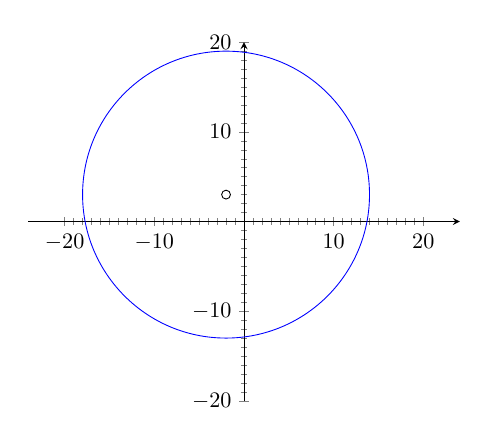
\begin{tikzpicture}[scale=0.8]
    \begin{axis}[
        axis equal,
        xmin=-20,
        xmax=20,
        xtick={-20,-10,0,10,20},
        ymin=-20,
        ymax=20,
        ytick={-20,-10,0,10,20},
        minor tick num=9,
        axis lines=middle,
        % extra tick style={grid=major},
    ]
      \draw[blue] \pgfextra{
        \pgfpathellipse{\pgfplotspointaxisxy{-2}{3}}
            {\pgfplotspointaxisdirectionxy{16}{0}}
            {\pgfplotspointaxisdirectionxy{0}{16}}
        };
      \addplot [only marks,mark=o] coordinates { (-2,3) } ;
    \end{axis}
    \end{tikzpicture}}

  \choice
    \fbox{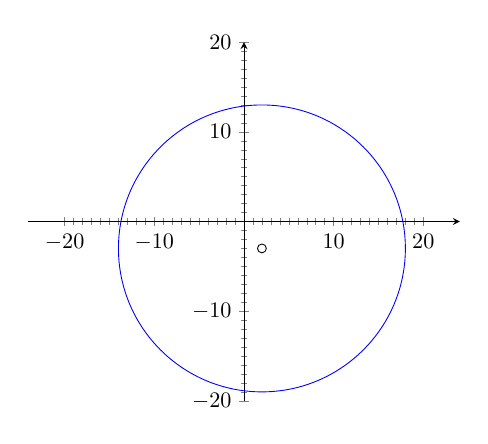
\begin{tikzpicture}[scale=0.8]
    \begin{axis}[
        axis equal,
        xmin=-20,
        xmax=20,
        xtick={-20,-10,0,10,20},
        ymin=-20,
        ymax=20,
        ytick={-20,-10,0,10,20},
        minor tick num=9,
        axis lines=middle,
        % extra tick style={grid=major},
    ]
      \draw[blue] \pgfextra{
        \pgfpathellipse{\pgfplotspointaxisxy{2}{-3}}
            {\pgfplotspointaxisdirectionxy{16}{0}}
            {\pgfplotspointaxisdirectionxy{0}{16}}
        };
      \addplot [only marks,mark=o] coordinates { (2,-3) } ;
    \end{axis}
    \end{tikzpicture}}

  \columnbreak

  \choice
    \fbox{\begin{tikzpicture}[scale=0.8]
    \begin{axis}[
        axis equal,
        xmin=-11,
        xmax=11,
        xtick={-10,-5,0,5,10},
        ymin=-11,
        ymax=11,
        ytick={-10,-5,0,5,10},
        minor tick num=4,
        axis lines=middle,
        % extra tick style={grid=major},
    ]
      \draw[blue] \pgfextra{
        \pgfpathellipse{\pgfplotspointaxisxy{-2}{3}}
            {\pgfplotspointaxisdirectionxy{4}{0}}
            {\pgfplotspointaxisdirectionxy{0}{4}}
        };
      \addplot [only marks,mark=o] coordinates { (-2,3) } ;
    \end{axis}
    \end{tikzpicture}}

  \choice
    \fbox{\begin{tikzpicture}[scale=0.8]
    \begin{axis}[
        axis equal,
        xmin=-11,
        xmax=11,
        xtick={-10,-5,0,5,10},
        ymin=-11,
        ymax=11,
        ytick={-10,-5,0,5,10},
        minor tick num=4,
        axis lines=middle,
        % extra tick style={grid=major},
    ]
      \draw[blue] \pgfextra{
        \pgfpathellipse{\pgfplotspointaxisxy{2}{-3}}
            {\pgfplotspointaxisdirectionxy{4}{0}}
            {\pgfplotspointaxisdirectionxy{0}{4}}
        };
      \addplot [only marks,mark=o] coordinates { (2,-3) } ;
    \end{axis}
    \end{tikzpicture}}

  \choice None of these.

\end{checkboxes}
\end{multicols}

\question[15]
Which of the following equations corresponds to the parabola sketched here?

\begin{center}
    \fbox{\begin{tikzpicture}[scale=0.8]
    \begin{axis}[
        axis equal,
        xmin=-11,
        xmax=11,
        xtick={-10,-5,0,5,10},
        ymin=-11,
        ymax=11,
        ytick={-10,-5,0,5,10},
        minor tick num=4,
        axis lines=middle,
        % extra tick style={grid=major},
    ]
      \draw[blue] \pgfextra{
        \pgfpathellipse{\pgfplotspointaxisxy{2}{-3}}
            {\pgfplotspointaxisdirectionxy{4}{0}}
            {\pgfplotspointaxisdirectionxy{0}{4}}
        };
      \addplot [only marks,mark=o] coordinates { (2,-3) } ;
    \end{axis}
    \end{tikzpicture}}
\end{center}

\end{questions}





\newpage


\begin{center}
  \textbf{Full Response (100 points total)}
\end{center}

\begin{questions}

\setcounter{question}{0}

\question[5]
  Compute the angle between the vectors
  $\vect{u}=\<2,2\sqrt{3}\>$ and $\vect{v}=\<-5,0\>$.

\newpage

\question[5]
  Find an equation for the plane passing through $(0,0,0)$,
  $(1,0,-3)$, and $(-2,3,0)$.

\newpage

\question[5]
  Sketch $x^2+9y^2-4z^2=16$ and its traces in the planes $x=0$, $y=0$,
  and $z=0$.
  Then use these traces to name the quadric surface.

\newpage

\question[5]
  Explain why the parametric equations $x=4\sin t$ and $y=\cos t$
  yield points on the ellipse $x^2+16y^2=16$.

\newpage

\question[5]
  Find $\vect{r}(t)$ given
  $\vect{r}'(t) = \left\<4t^3, -\sin t, e^t\right\>$
  and $\vect{r}(0) = \<1, 2, 3\>$.

\newpage

\question[5]
  Recall from the notes that the work done by moving an object
  along the displacement vector $\vect{D}$ using a force vector
  $\vect{F}$ is given by
  \[
    W = \vect{F}\cdot\vect{D}
  \]

  Use this formula to show how much work is done in moving an
  object from the point $(1,3)$ to the point $(4,7)$ using
  a force of magnitude $10$ units oriented
  in the positive $y$-direction.
\end{questions}

\end{document}